\subsection{Proximal Methods}
A possible solver is the Fast Iterative Shrinkage Tresholding Algorithm (\fista), first introduced in~\cite{fista}.
The discussion of \fista\ follows~\cite{fista}, the description of
the proximal operators follows~\cite{proxsurvey}.
\fista\ is able solve problems of the form
\begin{equation}\label{eq:composite-goal}
\min_{\bm{\alpha}} F(\bm{\alpha}) = f(\bm{\alpha}) + g(\bm{\alpha}),
\end{equation}
i.e.~minimizing functions that can be expressed as a sum of a convex, smooth function \(f(\bm{\alpha})\) and another convex, possibly non-smooth function \(g(\bm{\alpha})\).
It is required that \(f(\bm{\alpha})\) has a Lipschitz-continuous gradient. 
This means that the following condition holds for all possible vectors \(\bm{x}\) and \(\bm{y}\) for some positive constant \(L\):
\sidetitle{Lipschitz constant}
\begin{equation}   \label{eq:lipschitz}
 \Vert \bm{\nabla} f(\bm{x}) - \bm{\nabla} f(\bm{y}) \Vert \leq L \Vert \bm{x} - \bm{y} \Vert.
\end{equation}
We call the smallest possible value of \(L\) the Lipschitz constant.

For our goal given by \cref{eq:composite-goal} we set \(f(\bm{\alpha})\) to
\begin{equation*}
 f(\bm{\alpha}) = \frac{1}{2} \left\Vert  \bm{\Phi} \bm{\alpha} - \bm{y}   \right\Vert_2^2,
\end{equation*}
such that the gradient of \(f\) is then given by
\begin{equation*}
  \bm{\nabla} f(\bm{\alpha}) = \bm{\Phi}^\intercal \left(\bm{\Phi} \bm{\alpha} - \bm{y} \right).
\end{equation*}
The Lipschitz constant for the gradient of \(f\) is
\begin{equation}
  \label{eq:lipf}
  L_{\bm{\nabla} f} = {\left(\sigma_{\max} \left(\bm{\Phi}\right)\right)}^2,
\end{equation}
where \(\sigma_{\max} \) corresponds to the maximum singular value~\autocite{fista}.
Additionally we set \(g\) to
\begin{equation*}
  g(\bm{\alpha}, \lambda) = \mathcal{S} \left( \bm{\alpha}, \lambda \right).
\end{equation*}

We now define the Moreau envelope of a function \(g (\bm{\alpha})\), which is given for any \(\lambda \in (0, +\infty)\) by
\sidetitle{Moreau envelope}
\begin{equation}
  \label{eq:moreau-reg}
  M_{g}(\bm{\alpha}, \lambda) = \inf_{\bm{x}} \left\{  g(x) + (1/(2\lambda)) \Vert x - \bm{\alpha} \Vert_2^2 \right\}.
\end{equation}
It is a regularized, smooth version of our function \(g(\bm{\alpha})\) that has the
same minimum as \(g(\bm{\alpha})\).
That means, that every point that minimizes \(M_{g}(\bm{\alpha}, \lambda)\) also
minimizes our original function \(g (\bm{\alpha})\)~\cite{proxsurvey}.
Finally, we are able to define the proximal operator that returns the infinum
point of \cref{eq:moreau-reg} by
\begin{equation}
  \label{eq:proximal}
  \prox[\(g\)]{\bm{\alpha}}{\lambda}= \argmin_{\bm{x}} \left\{ g (\bm{x}) + (1/ (2 \lambda)) \Vert \bm{x} - \bm{\alpha} \Vert_2^2 \right\}.
\end{equation}
\sidetitle{Proximal Operator}
The proximal operator can be viewed as a gradient step with stepsize \(\lambda\) on the Moreau envelope
\(M_g(\bm{\alpha}, \lambda)\)
\begin{equation*}
  \prox[\(g\)]{\bm{\alpha}}{\lambda} = \bm{\alpha} - \lambda \bm{\nabla} M_{g}(\bm{\alpha}, \lambda).
\end{equation*}
This identity follows by rewriting \cref{eq:moreau-reg} in terms of the proximal operator and calculating the gradient~\cite{proxsurvey}.
We can use \cref{eq:proximal} to minimize \(M_g(\bm{\alpha}, \lambda)\) and
thus also for optimizing \(g(\bm{\alpha})\).
In the most general case \cref{eq:proximal} would imply the need to solve a convex optimization problem.
Fortunately we can find closed form solutions for many functions.
Consider for example \(g(\bm{\alpha}) = 0\).
In this case the Moreau envelope and the proximal operator are trivial
\begin{align*}
 M_{0}(\bm{\alpha}, \lambda) &= \inf_{\bm{x}} \left\{ 0 + 1/(2 \lambda) \Vert \bm{\alpha} - \bm{x} \Vert_2^2 \right\}, \\
 \prox[\(0\)]{\bm{\alpha}}{\lambda} &= \bm{\alpha}.
\end{align*}
It is obvious, that the minimum of \(M_g(\bm{\alpha}, \lambda)\) is equivalent to the minimum of \(g(\bm{\alpha})\), the proximal operator is corresponds to a gradient step on \(M_g\).

We are now going to develop a minimizer for our composite goal that resembles a majorization-minimization algorithm.
To do this, we first define an upper-bound of \(F(\bm{\alpha})\)~(\emph{majorizing}) that we are then going to minimize~(\emph{minimization})~\autocite{proxsurvey}.

\sidetitle{Upper Bound}
We first give a regularized linearization of \(f(\bm{\alpha})\) at an arbitrary,
but fixed point \(\bm{y}\) for an \(L > 0\):
\begin{equation}\label{eq:f-approx}
  \hat{f}_L(\bm{\alpha}, \bm{y}) = f(\bm{y}) + \left< \bm{\alpha} - \bm{y}, \bm{\nabla} f (\bm{y}) \right> +
  L/2 \Vert \bm{\alpha} - \bm{y} \Vert_2^2,
\end{equation}
where the angle brackets \( \left< \bm{x}, \bm{y} \right> = \bm{y}^\intercal \bm{x} \) represent the inner product.
The first two summation terms are given by the first order Taylor expansion of \(f(\bm{\alpha})\) at the point \(\bm{y}\), the last term can be interpreted as a trust-region or regularization, that punishes large deviations from~\(\bm{y}\)~\cite{proxsurvey}.
We then combine this linearization with our second function to archive an upper-bound of \(F(\bm{\alpha})\):
\begin{equation}\label{eq:goal-approx}
  Q_L(\bm{\alpha}, \bm{y}) = f(\bm{y}) + \left< \bm{\alpha} - \bm{y}, \bm{\nabla} f (\bm{y}) \right> +
  L/2 \Vert \bm{\alpha} - \bm{y} \Vert_2^2 +
  g(\bm{\alpha}).
\end{equation}
We can see from \cref{eq:lipschitz} that \(Q_L(\bm{\alpha}, \bm{y})\) is an
upper-bound of \(F(\bm{\alpha})\) iff.~L is equal to or greater than the Lipschitz
constant of \(\bm{\nabla} f(\bm{\alpha})\).

\sidetitle{Fixed-point minimizer}
The minimizer for this approximation is then given as the fixed-point equation
\begin{align}\label{eq:step}
  \pi_{g(\bm{\alpha})}(\bm{\alpha}^*, L) &=  \argmin_{\bm{x}} \left\{ Q_L(\bm{x}, \bm{\alpha}) \right\}\nonumber\\
       &= \prox[\(g\)]{\bm{\alpha^*} - L^{-1} \bm{\nabla} f (\bm{\alpha^*})}{L^{-1} } \nonumber\\
       &= \prox[\(g\)]{\bm{\alpha^*} - L^{-1} \bm{\Phi}^\intercal \left(\bm{\Phi} \bm{\alpha^*} - \bm{y} \right)}
         {L^{-1}},
\end{align}
where \(\bm{\alpha}^*\) denotes the optimal solution and \(L\) is the Lipschitz constant of \(\bm{\nabla} f\) given by \cref{eq:lipf}~\cite{fista}.
In this equation \(L\) is used to determine the optimal stepsize.
This minimizer is called proximal gradient algorithm or proximal-splitting in the literature, because we first perform a gradient step on \(f'_L(\bm{\alpha})\) given by~\ref{eq:f-approx} and then a proximal step on \(g(\bm{\alpha})\)~\cite{proxsurvey}.
Using \cref{eq:step} repeatedly on a point will result in the fixed-point, i.e.~the minimum of the upper bound, and thus also in the minimum of our original goal~\cite{proxsurvey}.

\begin{algorithm}
 \caption{Iterative Shrinkage Tresholding Algorithm (\ista)~\cite{fista}}\label{alg:ista} 
 \begin{algorithmic}[1]
   \Require{Lipschitz constant \(L\) of \(\bm{\nabla} f\), regularization parameter \(\lambda\)}
    \Statex
    \Function{Ista}{$L, \bm{\alpha}$} \Comment{\(\bm{\alpha}\) is an initial guess}
      \While{not converged}
        \Let{$\bm{\alpha}$}{\( \pi_{g(\bm{\alpha})} \left( \bm{\alpha}, L \right) \)}
      \EndWhile
     \State \Return{\(\bm{\alpha}\)}
    \EndFunction
\end{algorithmic}
\end{algorithm}

\Cref{eq:step} is all we need to define the simple iterative scheme called
Iterative Shrinkage Tresholding Algorithm~(\ista) as seen in \cref{alg:ista}.
Originally the name \ista\ was only used for solving the Lasso problem, but is now used for the more general algorithm as well. 
For our trivial function \(g(\bm{\alpha}) = 0\) this iterative scheme is identical to the standard gradient descent algorithm.

\sidetitle{Proximal Operators for Regularization}
So far we have only seen the proximal operator of a very simple function.
This is of course not satisfactory, the motivation for this chapter is solving the Lasso and the Elastic Net regularization problems.
Fortunately, closed form solutions for the other needed proximal operators exist as well:
\begin{align}
\label{eq:prox-lasso}
\text{for Lasso} \quad &&
    \left( \prox[\(\lambda \Vert \bm{\alpha} \Vert_1\)]{\bm{\alpha}}{t} \right)_i &= \left[\alpha_i - t \lambda \right]_+
    - \left[ -\alpha_i - t \lambda \right]_+, \\
\text{for Ridge} \quad &&
                          \left(  \prox[\( \lambda \Vert \bm{\alpha} \Vert_2^2\)]{\bm{\alpha}}{t} \right)_i &= (\alpha_i/(1 + 2t \lambda)), \nonumber\\
  \text{for Elastic Net} \quad && \prox[\( \lambda \Vert \bm{\alpha} \Vert_1 + \gamma \Vert \bm{\alpha} \Vert_2^2\)]{\bm{\alpha}}{t} &=
                                                                                                                                       \left( 1/(1 + 2 t \gamma) \right) \left(\prox[\(\lambda \Vert \bm{\alpha} \Vert_1\)]{\bm{\alpha}}{t}\right) \nonumber\\
  \text{for Group Lasso} \quad && {\left(\prox[\( \lambda \sum_{p \in \mathcal{P}} \sqrt{\vert p \vert} \Vert p \Vert_2 \)]{\bm{\alpha}}{t} \right)}_p &=
                                                                                     \left[ 1 - \left(\lambda t \sqrt{\vert p \vert}\right) \left( \Vert p \Vert_2 \right)^{-1} \right]_+ p \nonumber
\end{align}
where \( \left( x \right)_+ = \max(x, 0) \) denotes the positive part of \(x\)
and \(t\) is a stepsize.
The regularization parameters depend on the function \(g(\bm{\alpha})\).
We omit the derivations for the sake of brevity, the interested reader refers to the survey paper~\cite{proxsurvey}.
By setting the regularization parameter \(\lambda\) equal to zero, we recover, again, the gradient minimization method.

These proximal operators can be used to define a minimizer for a non-smooth
function \(g\).
\sidetitle{Minimizing Lasso}
For example, combining~\cref{eq:step} with the proximal operator for the
Lasso functional \(g(\bm{\alpha}) = \lambda \Vert \bm{\alpha} \Vert_1\) given by~\cref{eq:prox-lasso} results in
the minimizer
\begin{align*}
  \pi_{\lambda \Vert \bm{\alpha} \Vert_1}(\bm{\alpha^*} ,L)
  &=  \prox[\(\lambda \Vert \bm{\alpha} \Vert_1\)]{\bm{\alpha^*} - L^{-1} \bm{\nabla} f (\bm{\alpha^*})}{L^{-1}} \\
  &= {\left[ \left(\bm{\alpha^*} - L^{-1} \bm{\nabla} f (\bm{\alpha^*}) \right) - \lambda L^{-1} \right]}_+ -
    {\left[ -\left(\bm{\alpha^*} - L^{-1} \bm{\nabla} f (\bm{\alpha^*}) \right) - \lambda L^{-1} \right]}_+,
\end{align*}
again given as a fixed-point iteration.
In this equation the function \( \left[ x \right]_+ \) is applied element-wise on its input vector.
We can then use this minimizer with \cref{alg:ista} to compute a solution to
the Lasso problem.
The fixed-point equations for the Lasso and Elastic Net Regularization are
computed analogously.

\ista always converges to the global maximum, but only does so linearly~\cite{fista}.
To overcome this problem, Beck and Teboulle combined the \ista algorithm with
the accelerated gradient descent algorithm discovered by Nesterov. 
\sidetitle{Nesterov's accelerated gradient descent}
Nesterov's accelerated gradient descent is closely related to the ordinary
gradient descent algorithm.
The first step is identical, each following step carries some momentum of the
step before, thus stabilizing the procedure.
It is an optimal first-order optimization schema, i.e.~one that cannot be
improved asymtotically.
It archives quadratic convergence.
This property is retained when combined with the proximal-splitting procedure \cref{alg:ista}, the result is called \fista~\cite{fista}.
Each step of \fista\ evaluates the gradient and the proximal operator once, just as \ista does.
This means that the accelerated algorithm has a comparable cost for each iteration.

Another problem with \cref{alg:ista} is its dependence on the Lipschitz constant of
\(\bm{\nabla} f\) to determine the optimal stepsize.
\sidetitle{Linesearch}
For our choice of \(f\), the best constant \(L\) is given by~\cref{eq:lipf}.
To avoid this expensive calculation, we use a backtracking line search to
determine a suitable stepsize.
In this line search procedure we use \cref{eq:goal-approx} as an upper bound for \cref{eq:composite-goal}.
We do this by iterating and finding the smallest \(L\) for which
\cref{eq:goal-approx} is an upper bound.
This always results in the Lipschitz constant~\cite{fista}.
It is then straightforward to derive \cref{alg:linesearch}.

\begin{algorithm}[h!]
 \caption{Linesearch~\cite{fista}}\label{alg:linesearch}
 \begin{algorithmic}[1]
  \Require{\(L > 0, \eta > 1, \bm{\alpha}\)} 
  \Statex
  \Function{Linesearch}{$\bm{\alpha}, L$}
    \Let{\(i\)}{\(0\)}
    \Do
      \Let{L}{\(\eta^i L\)}
      \Let{prox}{\(\pi_{\bm{\alpha}} (\bm{\alpha}, L)\)}
      \Let{\(i\)}{\(i + 1\)}
    \doWhile{$F(\text{prox}) < Q_L(\text{prox}, \bm{\alpha})$}
    \State \Return{prox and \(L\)} \Comment{Also return prox to avoid duplicate calculations.}
  \EndFunction
 \end{algorithmic}
\end{algorithm}

We need to evaluate the line search once for each iteration step.
It is possible that this procedure finds a non-optimal \(L\), i.e.~an \(L\) that
is larger than the Lipschitz constant.
This leads to a smaller stepsize, which is not a problem in practice, because
our optimization procedure still converges, although slower than possible.
We have to take that into consideration for our choice of linesearch parameters.
Usual values are \(L = 0.5\) and~\(\eta = 2\).
Using \cref{alg:linesearch} we can finally present an optimal first order optimization algorithm, shown by \cref{alg:fista}.

It is of course possible to use a constant stepsize like in \cref{alg:ista}.
To do this, replace the line search with the minimal value of \(L\) and
calculate \(\pi(\bm{\alpha}, L)\) directly.
We can also integrate the linesearch into the \ista algorithm, by replacing the
fixed \(L\) with a call to the linesearch subroutine.
A comparison of the practical speed of \ista and \fista with constant stepsize can be seen in~\cref{fig:fista-convergence}.

An alternative backtracking scheme for \fista is offered in~\cite{fista-backtracking}.
It offers the same asymptotic convergence speed, but shows practical improvements for some minimization problems.

\begin{figure}[bt]
  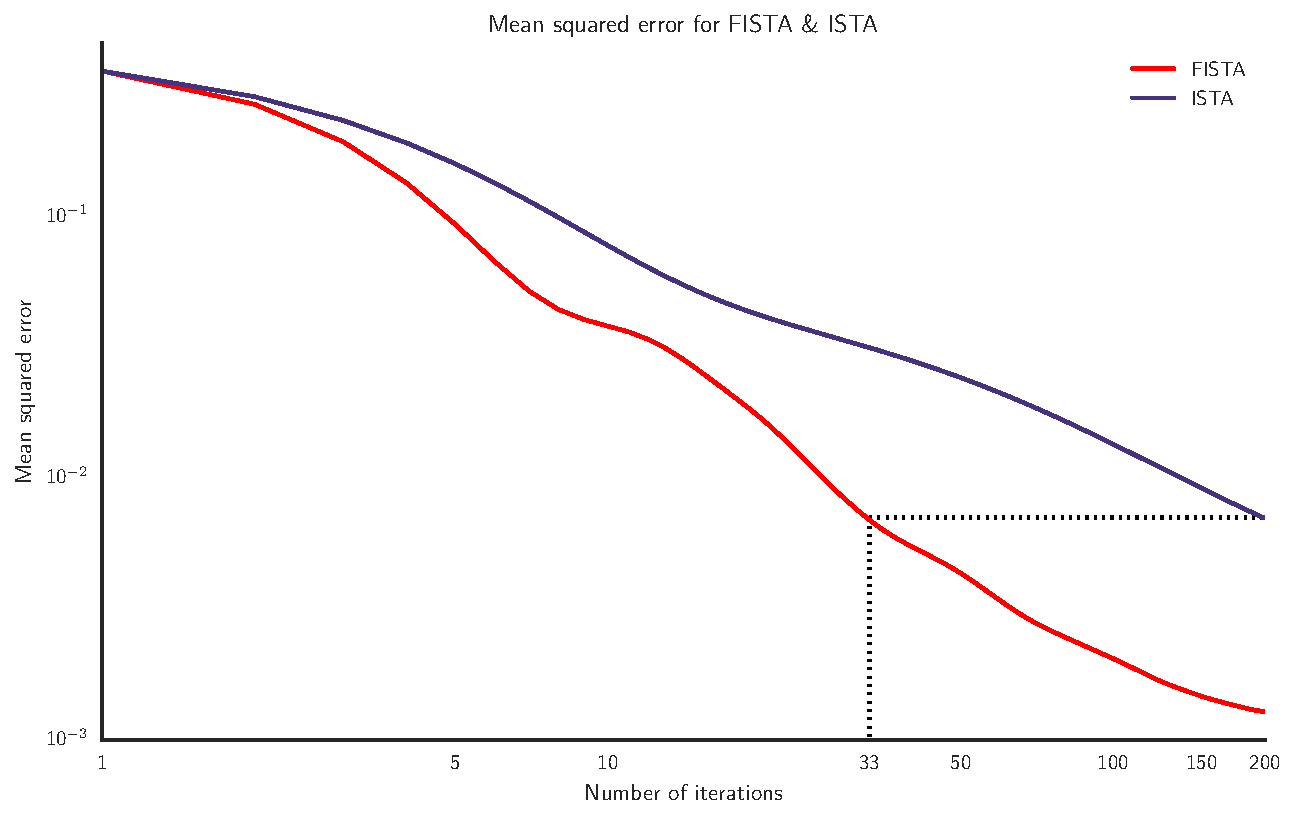
\includegraphics[scale=0.6]{fista}
  \caption[Comparison of \fista and \ista]{Comparison of \fista and \ista, both with constant stepsize.
    The figure shows the training mean squared error for the first 200
    iterations with \(\lambda = 0\) for the training set of the concrete
    data set.
    The dotted lines indicate the best value reached by \ista.
    Notice that \fista is able to return a better result after only 33
    iterations ---
    a drastic speedup compared to the 200 needed by \ista!
  }\label{fig:fista-convergence}
\end{figure}

\begin{algorithm}[h]
 \caption{Fast Iterative Shrinkage Tresholding Algorithm (\fista)~\cite{fista}} \label{alg:fista} 
 \begin{algorithmic}[1]
   \Require{Initial guess for Lipschitz constant \(L\) of \(\bm{\nabla} f\), regularization parameter \(\lambda\)}
    \Statex
    \Function{Fista}{$L, \bm{\alpha}$} \Comment{\(\bm{\alpha}\) is an initial
      guess for \(\alpha^*\).}
      \Let{\(\bm{y}\)}{\(\bm{\alpha}\)}
      \Let{\(t\)}{\(1\)}
      \While{not converged}
        \Let{\(\bm{\alpha}_{\text{before}} \)}{\(\bm{\alpha}\)}
        \Let{$\bm{\alpha}, L$}{\Call{Linesearch}{$ \bm{y}, L$ }} \Comment{Linesearch returns \(\pi_L (\bm{y})\) and the used L.}
        \Let{\(t_\text{before}\)}{\(t\)}
        \Let{\(t\)}{\(\nicefrac{1}{2} (1 + \sqrt{1+4t^2}) \)}
        \Let{\(\bm{y}\)}{\(\bm{\alpha} + \left( t_\text{before} -1 \right) t^{-1} 
                    \left(\bm{\alpha} - \bm{\alpha}_{\text{before}} \right)\)}
      \EndWhile
     \State \Return{\(\bm{\alpha}\)}
    \EndFunction
\end{algorithmic}
\end{algorithm}

%%% Local Variables:
%%% mode: latex
%%% TeX-master: "../main"
%%% End:
